% !TEX encoding = UTF-8
% !TEX TS-program = pdflatex
% !TEX root = ../relazione-finale.tex

%**************************************************************
\pagebreak
\chapter{Valutazione retrospettiva}
\label{cap:analisi-requisiti}
%**************************************************************

\section{Presentazione \emph{dashboard}}

Ho composto l'interfaccia grafica della \emph{dashboard} di due parti:
\begin{itemize}
  \item una barra verticale sulla sinistra contenente le voci di navigazione del menù;
  \item la restante parte della pagina per la visualizzazione dei contenuti.
\end{itemize}
Come illustro in figura ~\ref{fig:homepage}, nella pagina principale della \emph{dashboard} presento lo stato dei servizi del sistema: per ogni servizio mostro il nome, un icona di riconoscimento e, per mezzo di un pallino verde o rosso, il suo stato (operativo o malfunzionante).

\begin{figure}[!h]
    \centering
    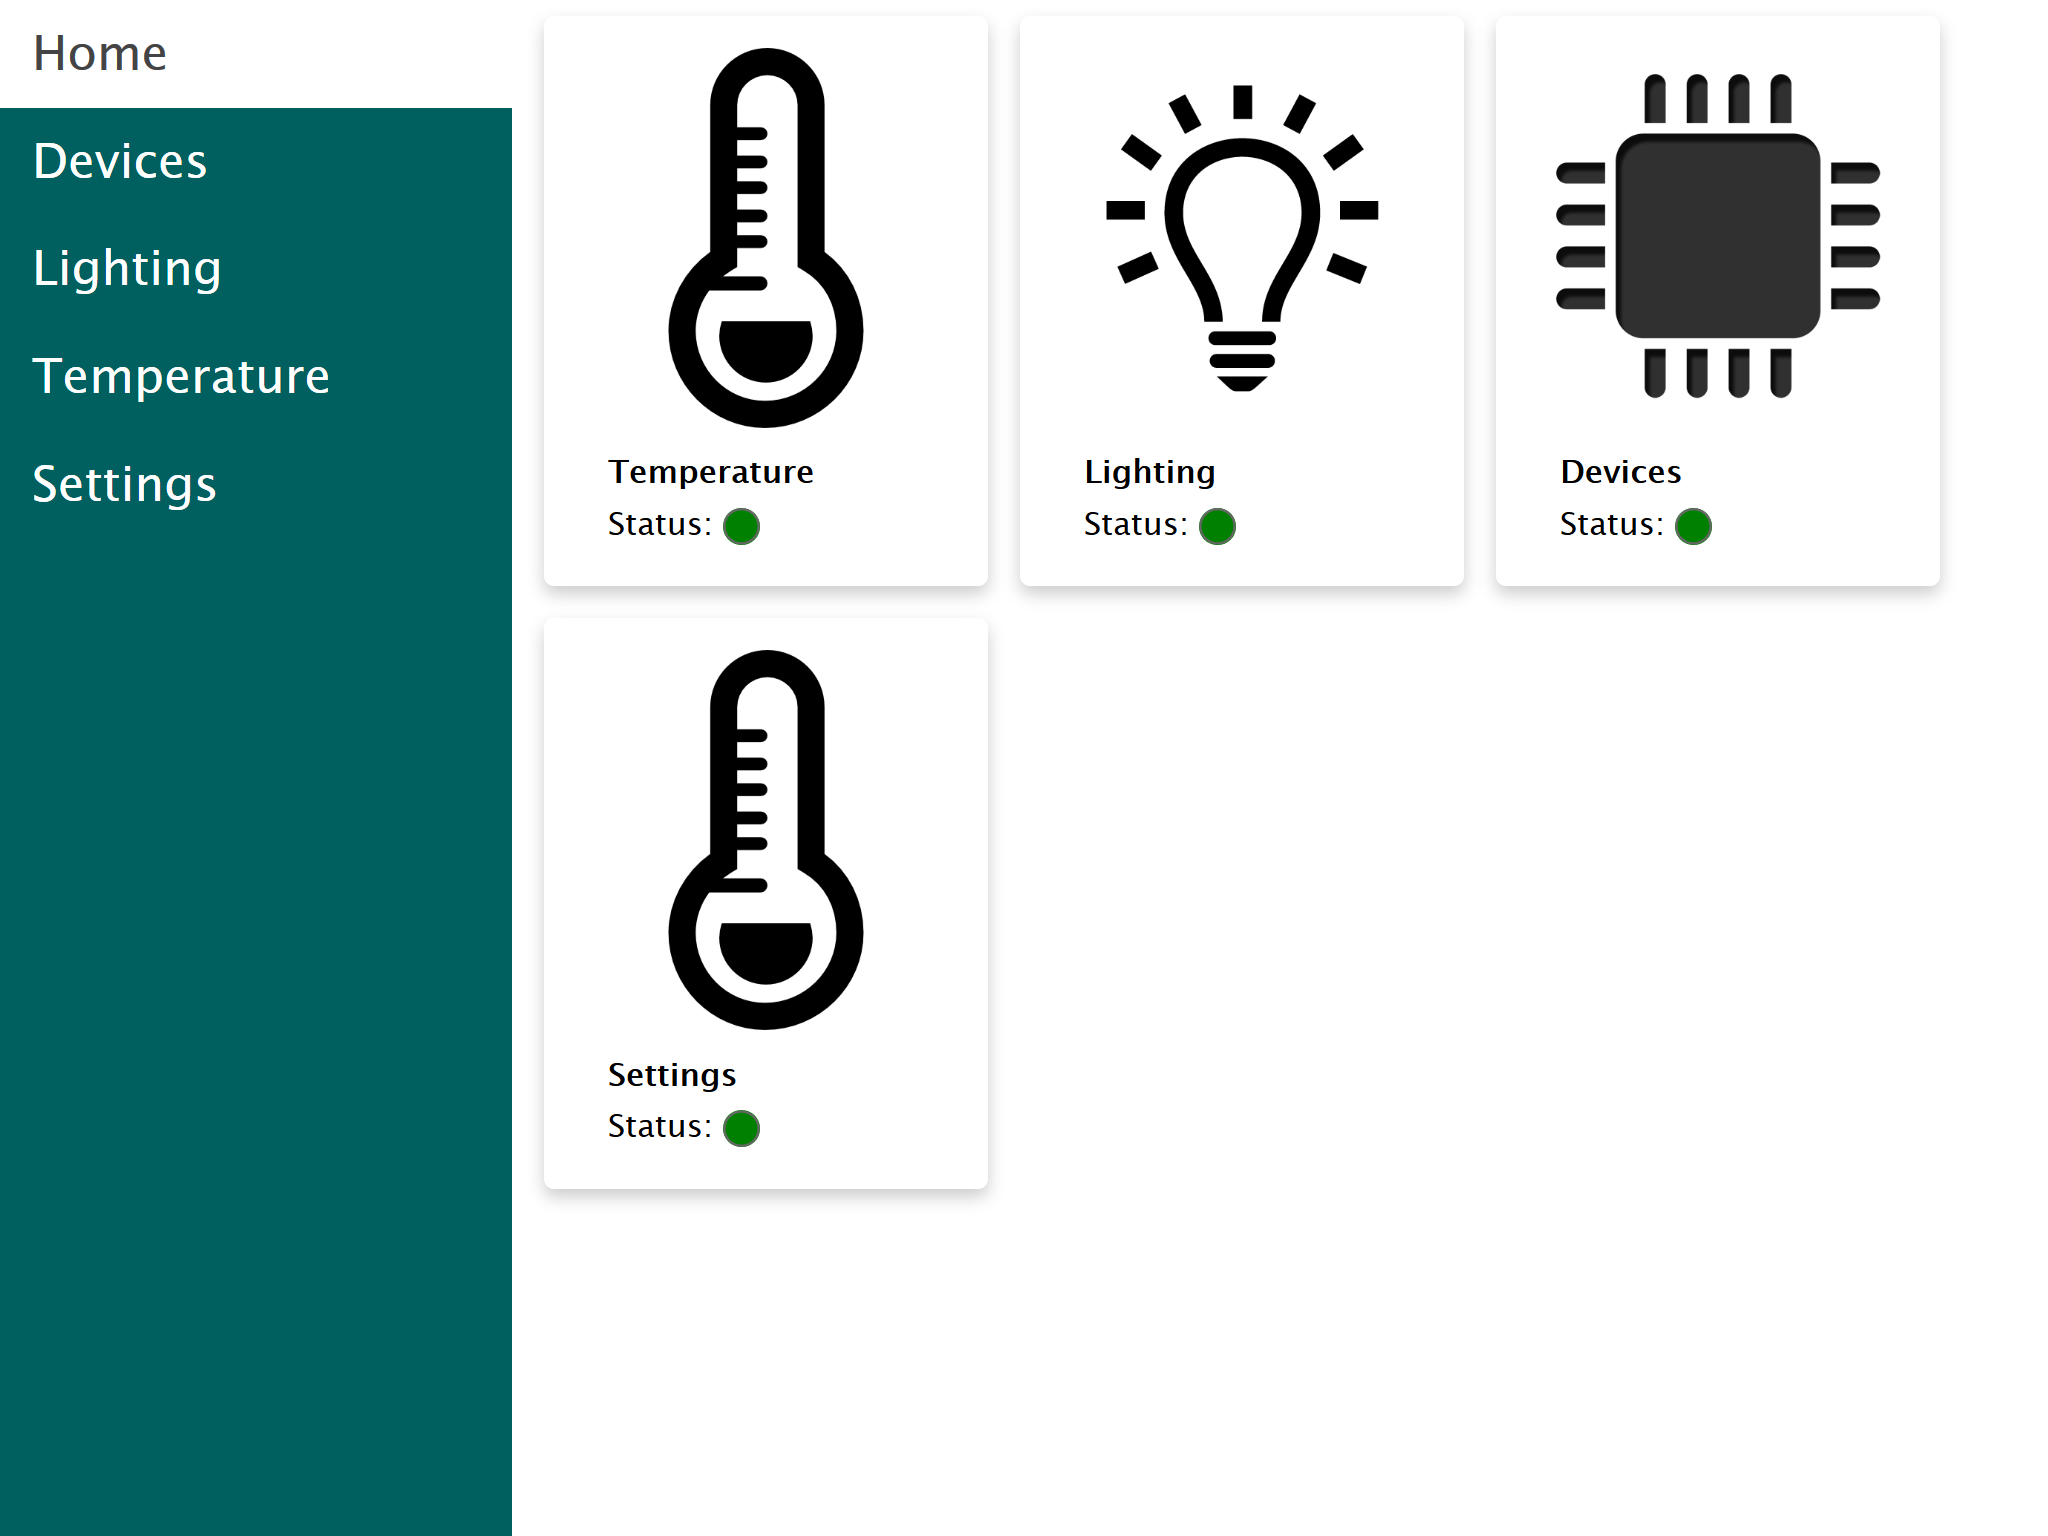
\includegraphics[width=0.9\columnwidth]{demo/home-page}
    \caption{Pagina principale della \emph{dashboard}}
    \label{fig:homepage}
\end{figure}

Navigando nella pagina dedicata ai dispositivi (voce \emph{Devices}), elenco i dispositivi collegati mostrandone la categoria, il produttore, il modello e la revisione. Ho inserito un'illustrazione di questa pagina in figura ~\ref{fig:devices}.

\begin{figure}[!h]
    \centering
    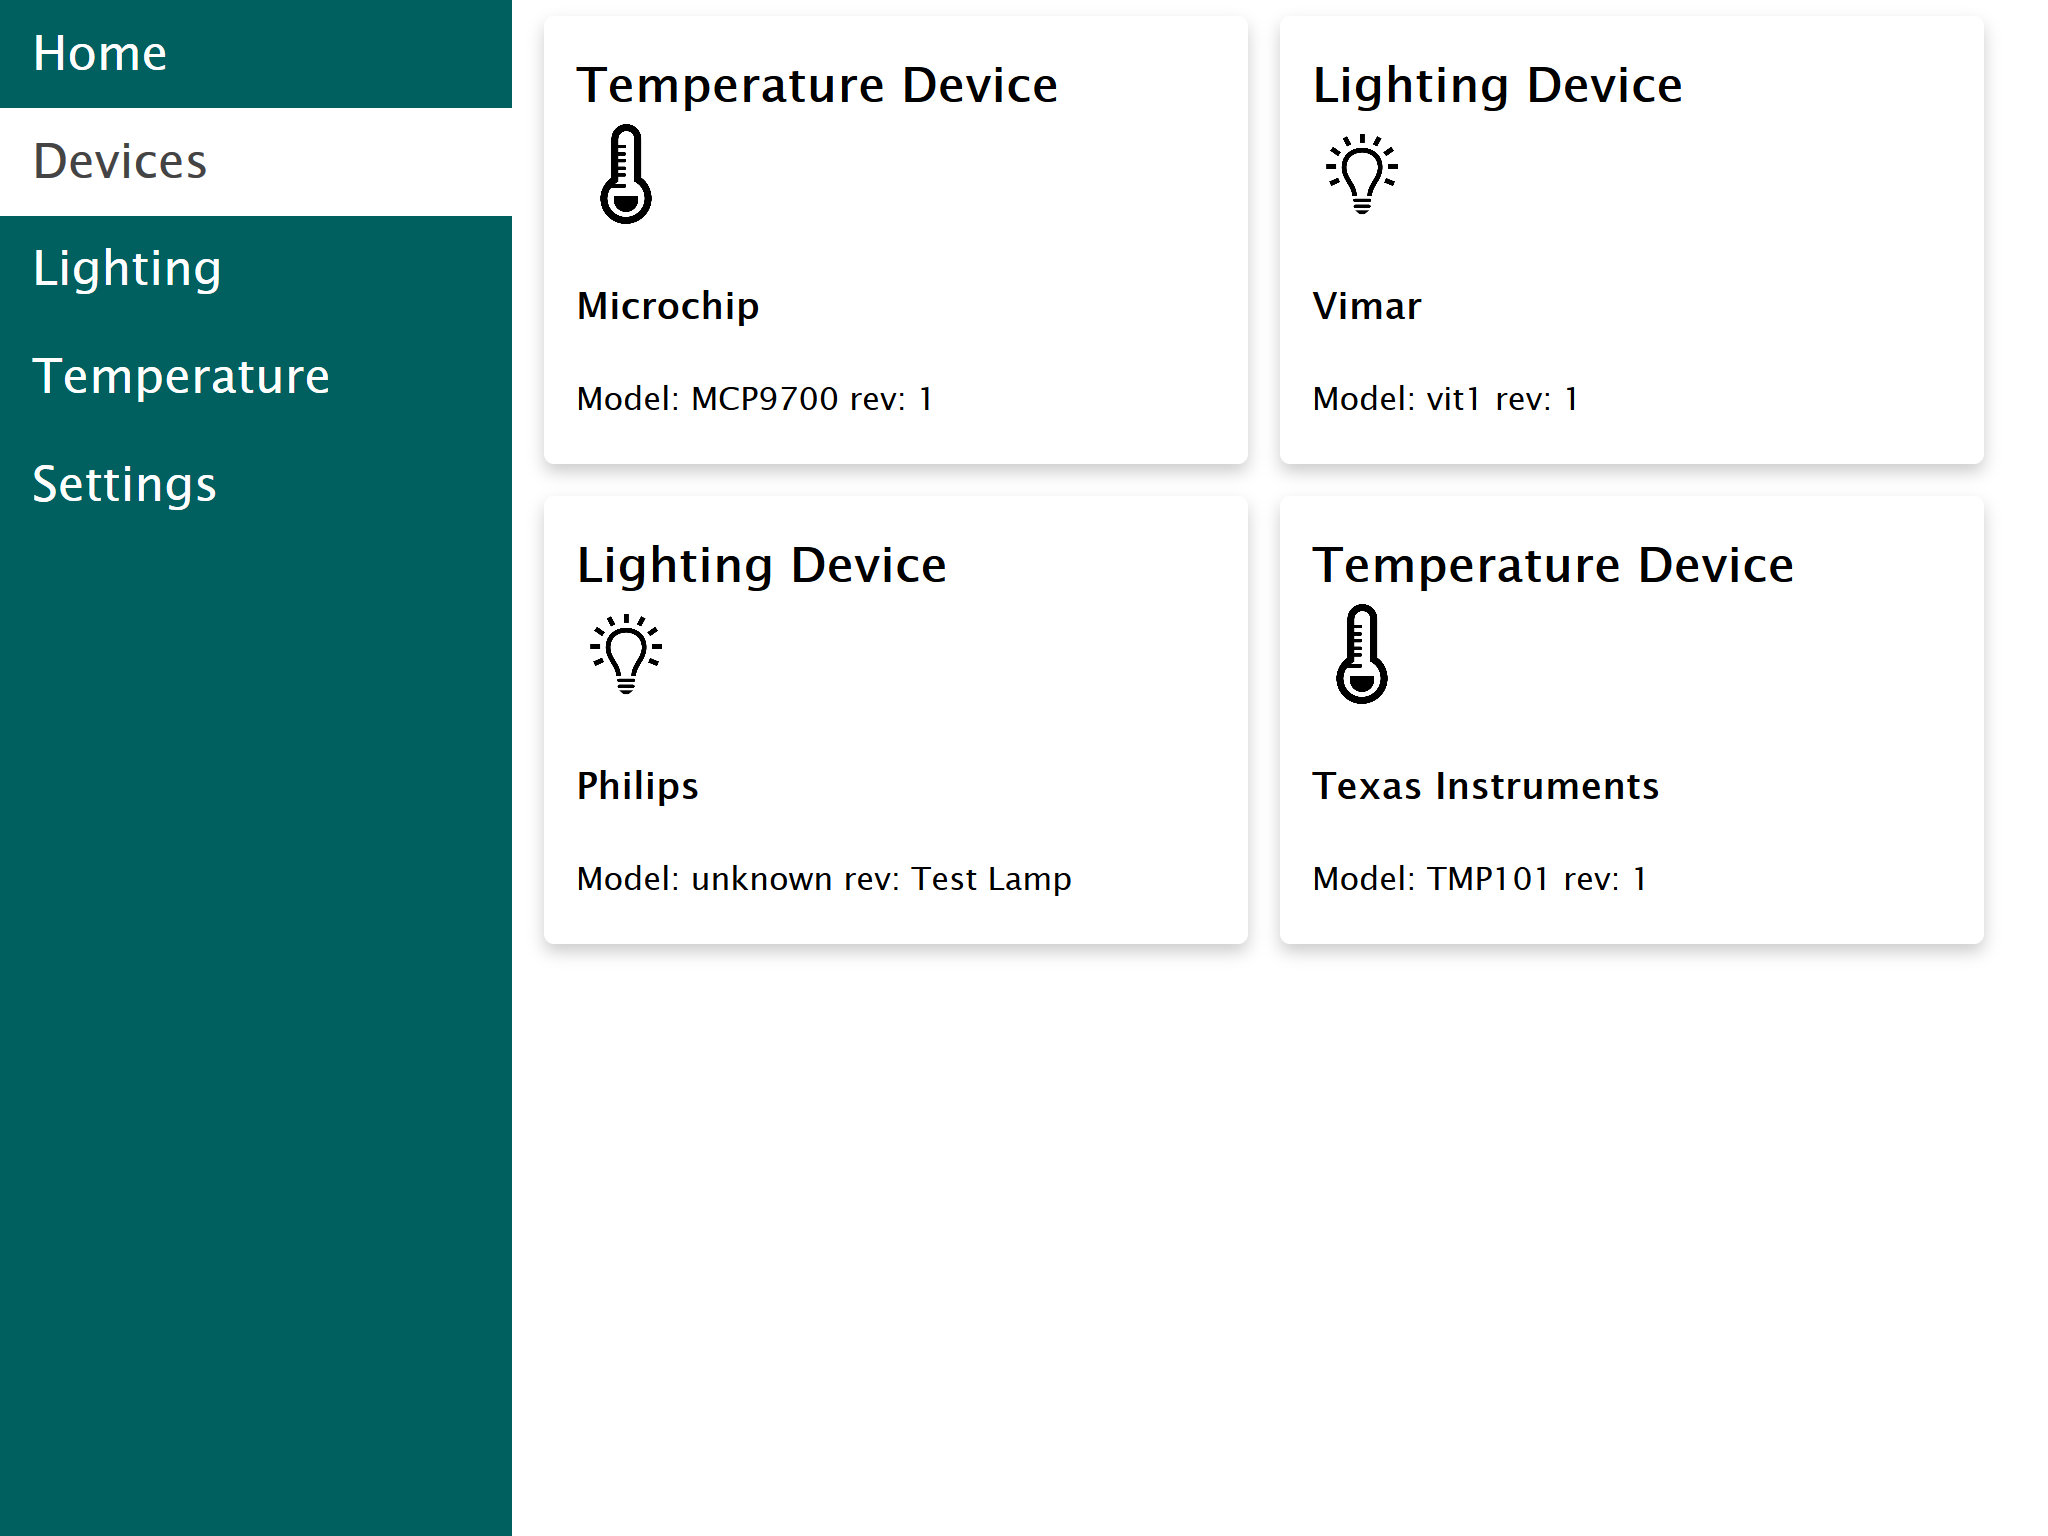
\includegraphics[width=0.9\columnwidth]{demo/devices}
    \caption{Pagina che ricapitola i dispositivi collegati alla \emph{dashboard}}
    \label{fig:devices}
\end{figure}

Nella pagina dedicata alle aree tematiche legate all'illuminazione e alla temperatura, riprendo la visualizzazione mostrata per l'elenco dei dispositivi collegati, mostrando solamente i dispositivi di quella categoria. Nel caso della pagina legata alla temperatura, per ogni dispositivo visualizzo l'identificativo del dispositivo, l'ultima temperatura rilevata e la data in cui il sensore ha misurato quella temperatura. Nella pagina legata all'illuminazione espongo per ogni dispositivo l'identificativo e la data dell'ultima comunicazione con la lampada.
Selezionando uno dei dispositivi elencati, apro una pagina di dettaglio in cui presento le ultime misurazioni disponibili (fino a 50) in un grafico.
Come è possibile osservare in figura ~\ref{fig:temp}, nella pagina di dettaglio di un sensore di temperatura visualizzo il suo identificativo, il produttore, il modello, la revisione e un grafico con l'andamento della temperatura rilevata dal dispositivo.
Ho implementato una funzionalità di personalizzazione dell'unità di misura per la temperatura: l'utente, accedendo alla pagina \emph{Settings}, può scegliere l'unità di misura della temperatura tra quelle gestite dal sistema. Quando l'utente cambia l'unità di misura, questa modifica si ripercuote su tutte le misurazioni di temperatura visualizzabili nella \emph{dashboard}, inclusi i grafici della temperatura.

\begin{figure}[!h]
    \centering
    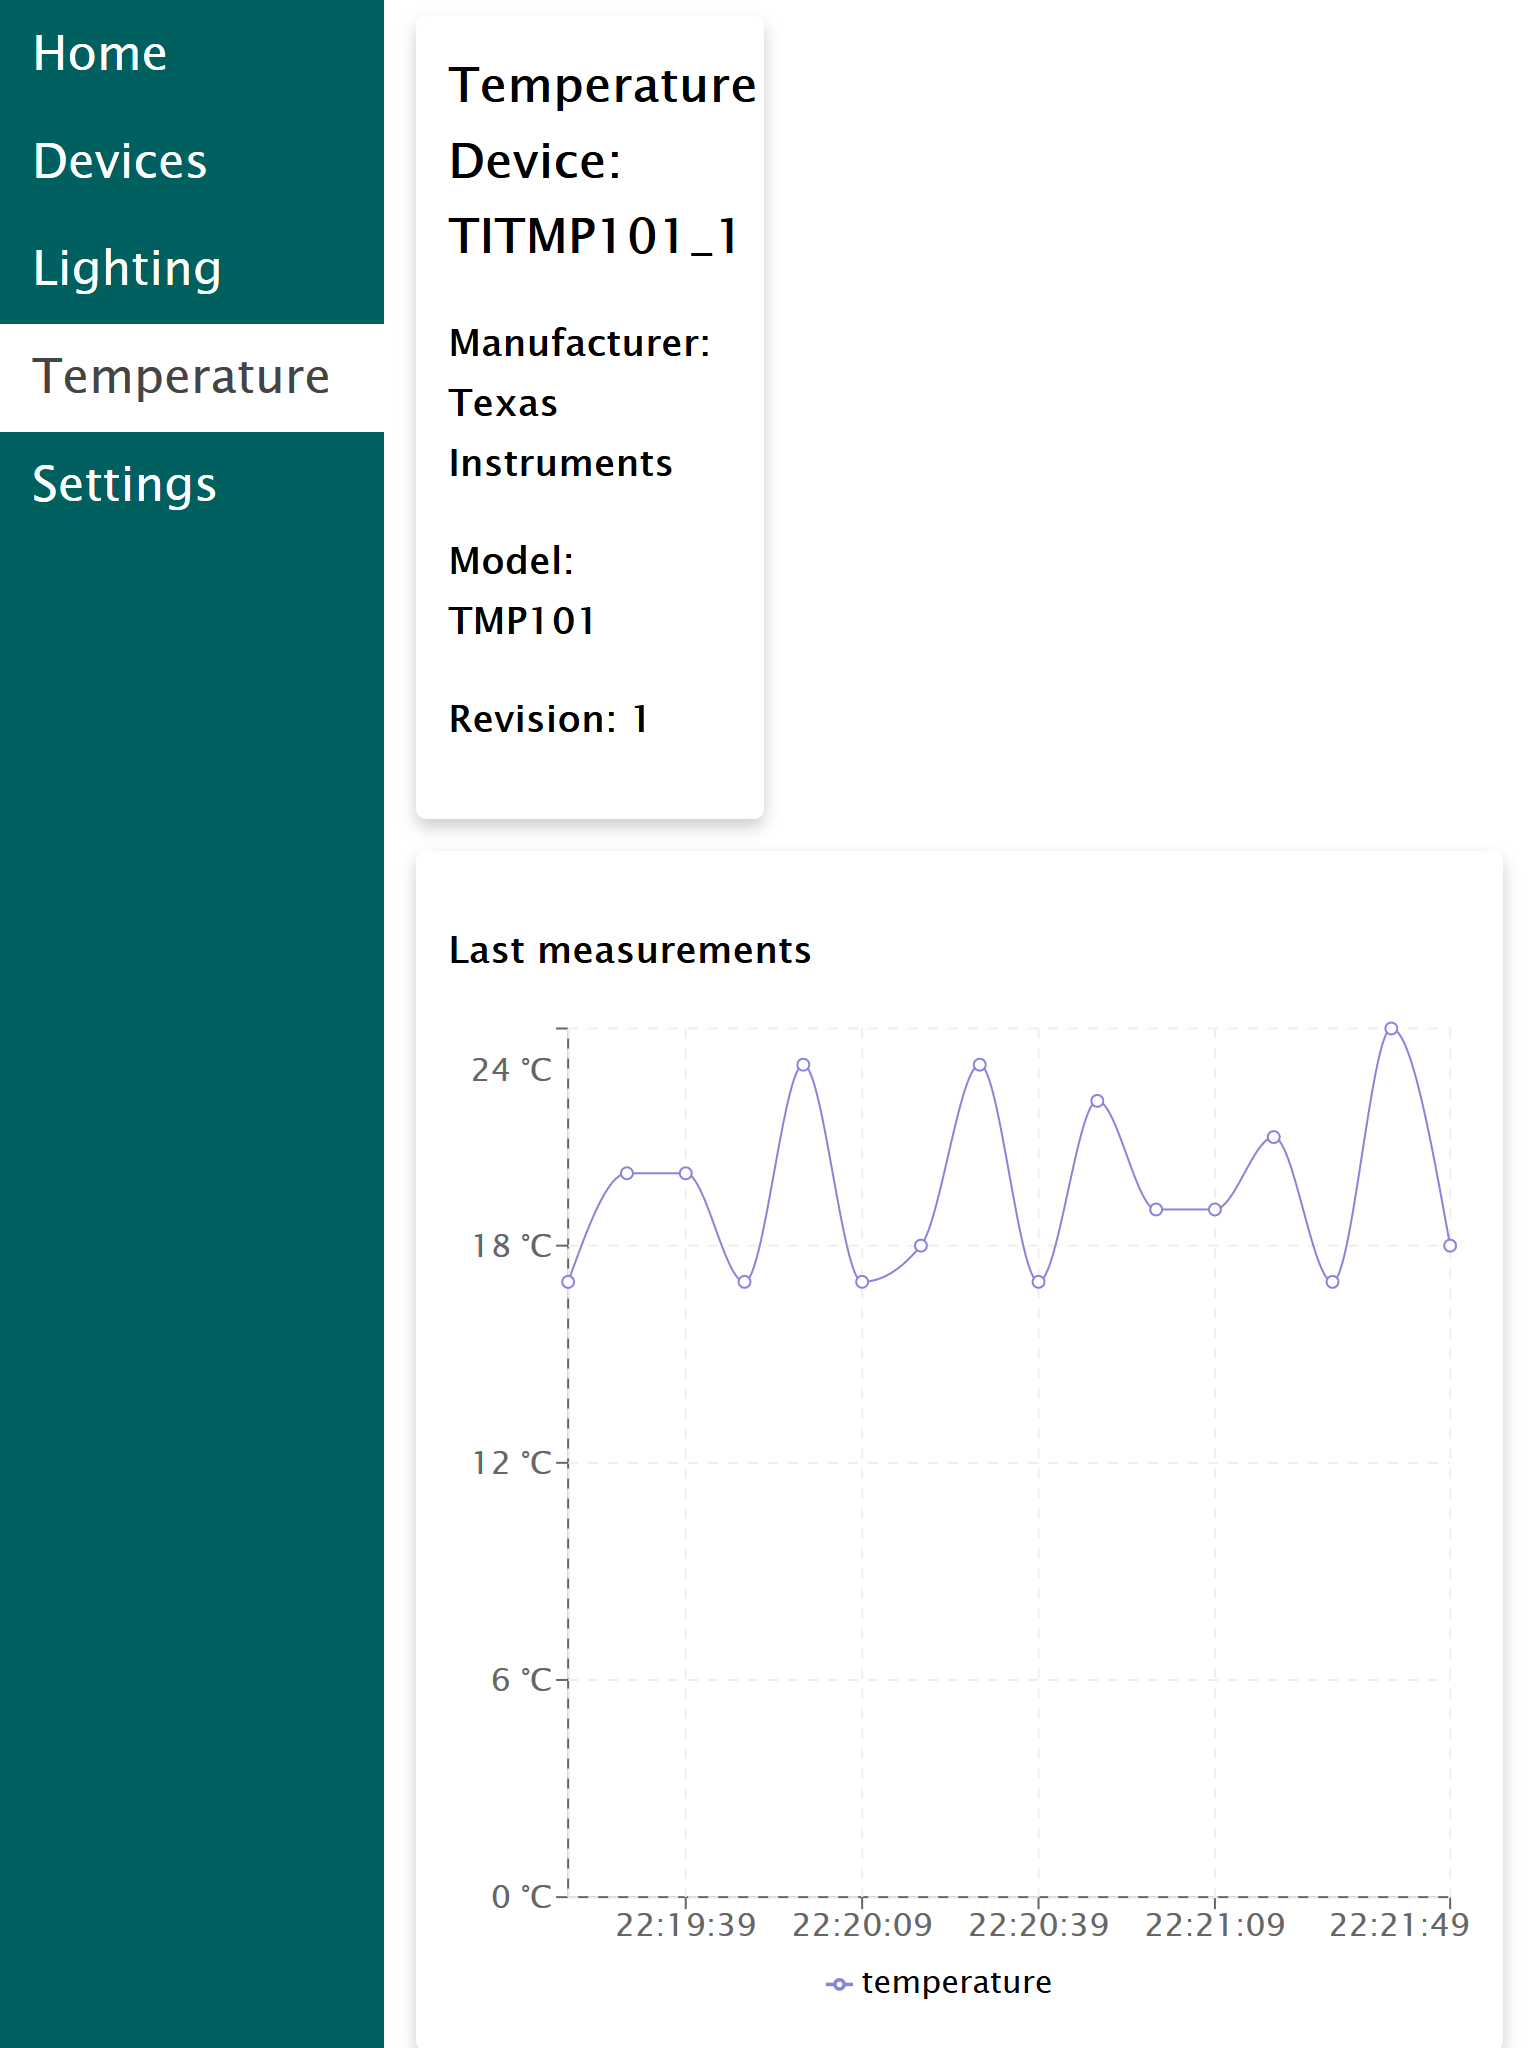
\includegraphics[width=0.6\columnwidth]{demo/ti-temperature}
    \caption{Pagina con il dettaglio di un sensore di temperatura}
    \label{fig:temp}
\end{figure}

Nella pagina di dettaglio delle lampade controllabili da remoto, presento le informazioni già citate con l'aggiunta di un interruttore per l'accensione e lo spegnimento della lampada. In questo caso nel grafico con le misurazioni indico sulle ordinate la potenza assorbita dalla lampada, secondo specifica del dispositivo. Ho incluso in figura ~\ref{fig:light} una schermata della pagine di dettaglio con la lampada spenta e in figura ~\ref{fig:light-on} una schermata della stessa pagina con la lampada accesa.

\begin{figure}[H]
    \centering
    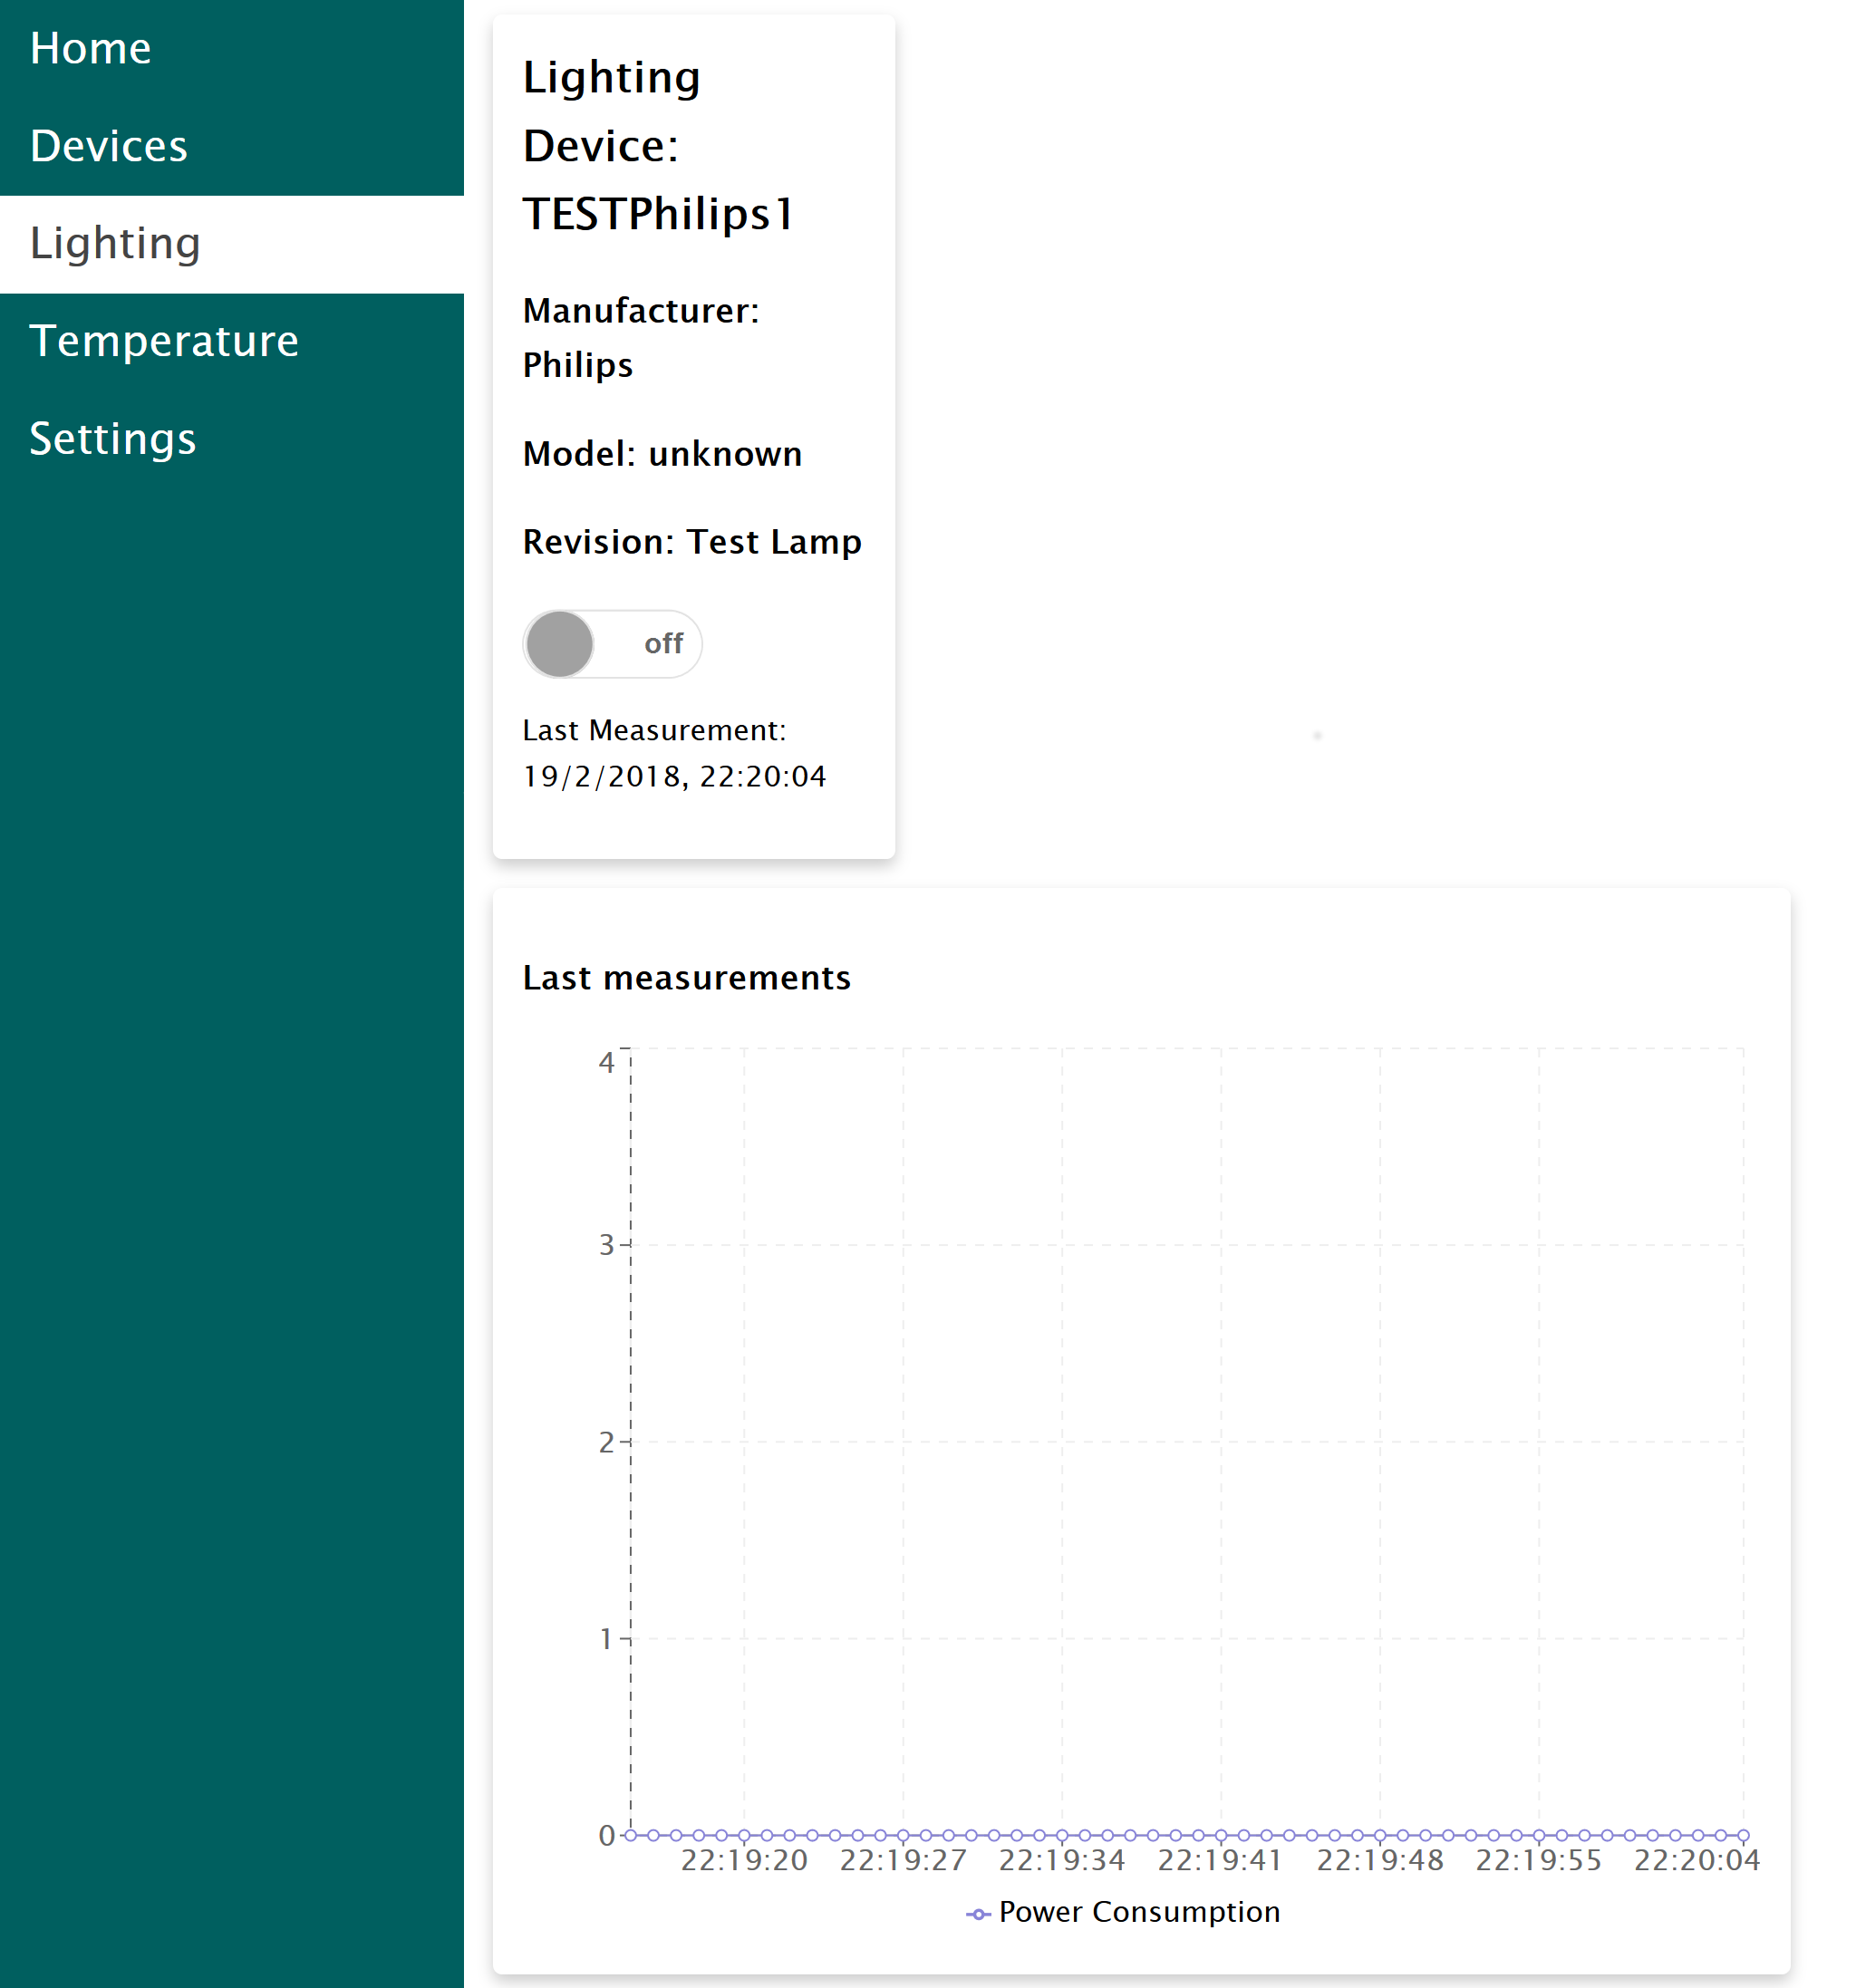
\includegraphics[width=0.6\columnwidth]{demo/philips-light}
    \caption{Pagina di dettaglio della lampada spenta}
    \label{fig:light}
\end{figure}

\begin{figure}[H]
    \centering
    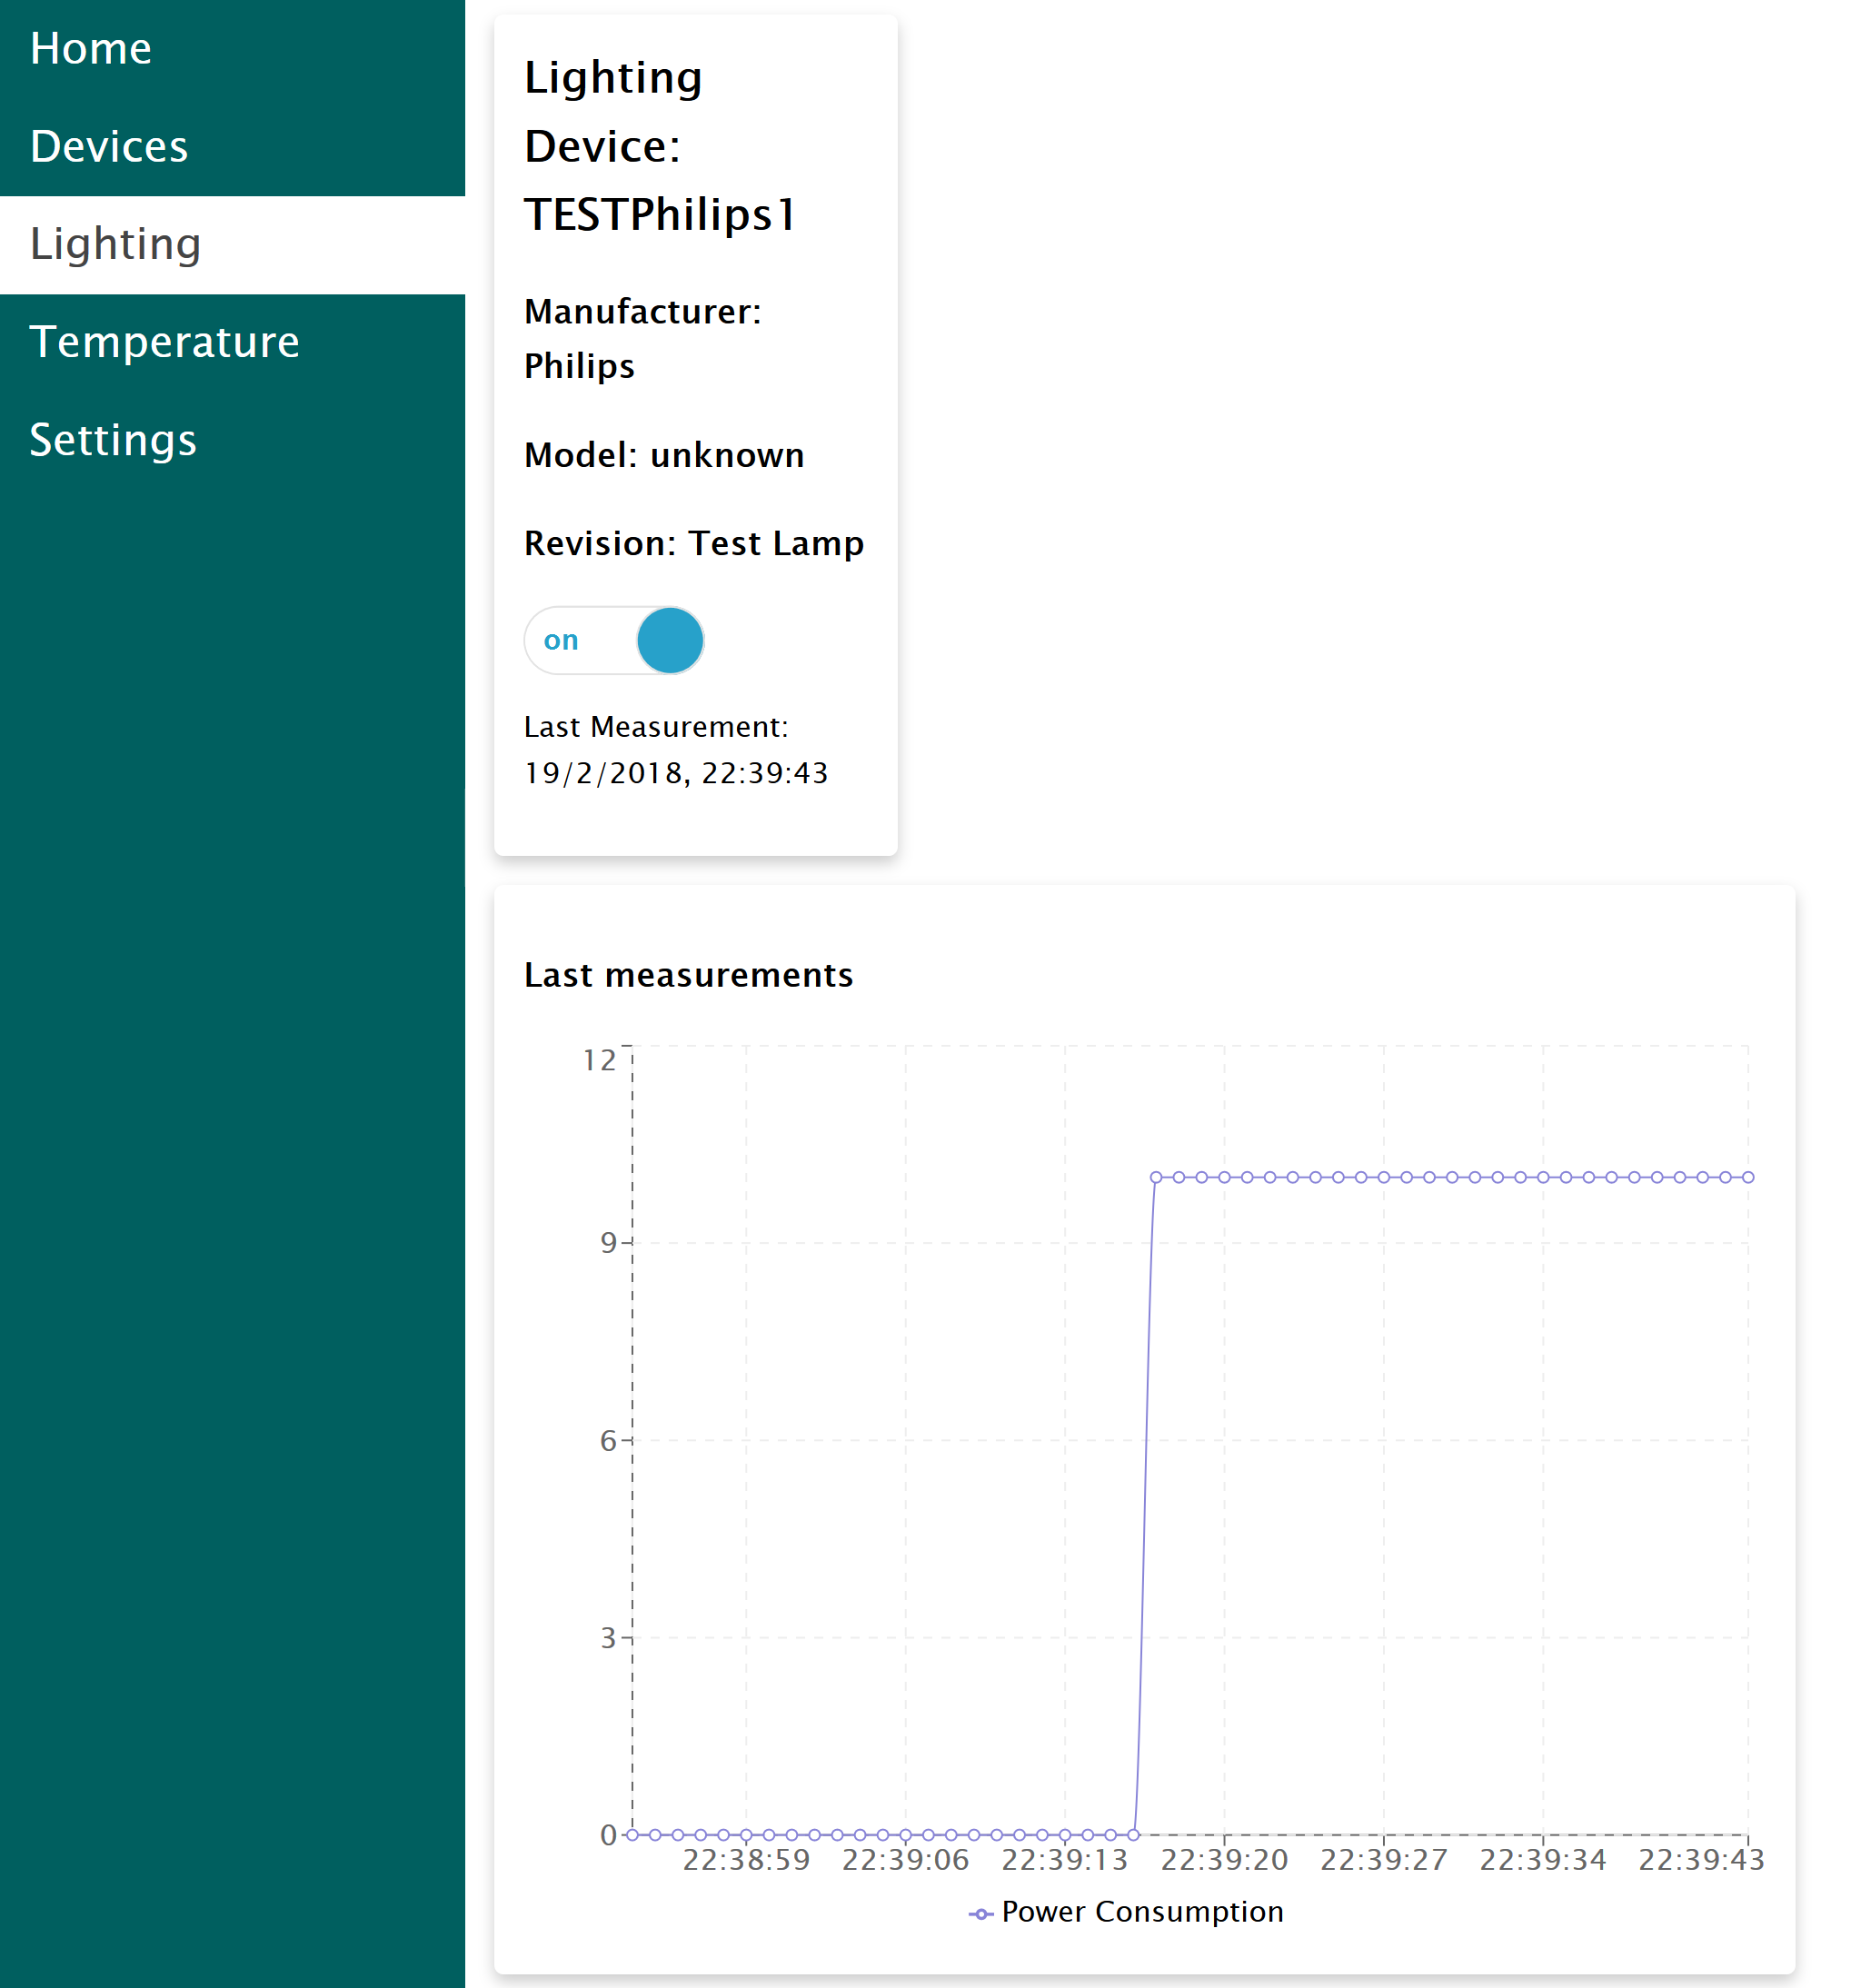
\includegraphics[width=0.6\columnwidth]{demo/philips-light-on}
    \caption{Pagina di dettaglio della lampada accesa}
    \label{fig:light-on}
\end{figure}

\section{Raggiungimento degli obiettivi}

Per valutare correttamente il raggiungimento degli obiettivi è necessario che riprenda gli obiettivi fissati nel capitolo ~\ref{cap:processi-metodologie}.
In particolare voglio osservare le tabelle in cui ho fissato gli obiettivi di prodotto (~\ref{tab:obiettivi-prodotto}), gli obiettivi formativi (~\ref{tab:obiettivi-formativi}) e tecnici (~\ref{tab:obiettivi-tecnici}) del progetto.

Iniziando dalla valutazione degli obiettivi di prodotto, posso definirmi soddisfatto delle funzionalità implementate nel prototipo.
Ho soddisfatto gli obiettivi "OP2" e "OP3", a cui avevo assegnato importanza critica, e quindi il prototipo mostra correttamente quello che mi aspettavo di presentare.
L'utente della \emph{dashboard} del prototipo può visualizzare correttamente la lista di dispositivi collegati al sistema e, per ciascuno di essi, può vedere:
\begin{itemize}
  \item le specifiche generali che comprendono:
  \begin{itemize}
    \item nome del dispositivo;
    \item produttore del dispositivo;
    \item revisione del dispositivo;
  \end{itemize}
  \item le ultime misurazioni provenienti dal dispositivo, nell'unità di misura scelta dall'utente;
  \item se il dispositivo presenta funzionalità \emph{smart}, elementi grafici che permettono all'utente di avviare tali funzionalità.
\end{itemize}
Ho parzialmente implementato le funzionalità descritte negli obiettivi "OP1" e "OP5".
Per quanto riguarda "OP1", nella pagina principale della \emph{dashboard} l'utente può osservare lo stato dei servizi che compongono il sistema, tuttavia considero questo obiettivo solamente parzialmente soddisfatto perché mi aspettavo di riuscire a visualizzare maggiori informazioni, come ad esempio le statistiche del traffico dati all'interno della rete.
Per quanto riguarda "OP5", l'utente può accedere a una pagina in cui può solamente cambiare due opzioni:
\begin{itemize}
  \item il proprio nome nel sistema;
  \item l'unità di misura della temperatura, utile nella visualizzazione delle temperature rilevate dai dispositivi legati a questo ambito.
\end{itemize}
Considero l'obiettivo "OP5" solamente parzialmente soddisfatto in quanto all'inizio del progetto mi aspettavo di riuscire a includere più opzioni di personalizzazione per l'utente.
L'omissione dell'obiettivo "OP4" e la parziale implmentazione di "OP5" e "OP1" è stata causata da due fattori:
\begin{itemize}
  \item difficoltà nelle attività di implementazione, citate in ~\ref{val-req};
  \item sottovalutazione dell'impegno richiesto per implementare le funzionalità più importanti.
\end{itemize}
Considero che le difficoltà implementative che ho riscontrato siano state causate dalla mia inesperienza con la realizzazione di architetture \emph{software} distribuite e dalla mancanza di documentazione che illustri le \emph{best practice} applicate in sistemi reali.
Nella tabella ~\ref{tab:esito-obiettivi-prodotto} riassumo la valutazione degli obiettivi di prodotto soddisfatti.

\begin{table}[H]
\caption{Tabella di valutazione delle funzionalità implementate nel prototipo}
\label{tab:esito-obiettivi-prodotto}
\begin{tabularx}{\linewidth}{|c|X|c|}
\hline
\textbf{Id obiettivo} & \textbf{Descrizione obiettivo} & \textbf{Esito}\\
\hline
OP1 & Visualizzare lo stato generale del sistema. & Parzialmente soddisfatto \\
\hline
OP2 & Visualizzare quali dispositivi sono collegati al sistema. & Soddisfatto \\
\hline
OP3 & Visualizzare le informazioni trasmesse dai dispositivi collegati al sistema. & Soddisfatto \\
\hline
OP4 & Implementare sistemi di autenticazione dell'utente. & Omesso \\
\hline
OP5 & Visualizzare e gestire le preferenze dell'utente. & Parzialmente soddisfatto \\
\hline
\end{tabularx}
\end{table}

Ho inserito nella tabella ~\ref{tab:esito-obiettivi-formativi} la mia valutazione degli obiettivi formativi del progetto.
Considero l'obiettivo "OF1" soddisfatto in quanto le attività di analisi svolte mi hanno permesso di individuare le funzionalità di dispositivi IoT che corrispondono a prodotti esistenti, confermando di fatto che le funzionalità che ho individuato sono richieste dal mercato.
Considero l'obiettivo "OF2" soddisfatto in quanto durante le attività di analisi ho individuato quali caratteristiche di prestazioni e affidabilità sono richieste da dispositivi con risorse di elaborazione limitate ed ho associato queste caratteristiche a ciascun protocollo valutato per determinare quale soluzione tecnica adottare. Ho quindi imparato a valutare l'importanza delle tecniche di individuazione e correzione degli errori dal punto di vista \emph{software}, della gestione dell'instaurazione del collegamento tra i dispositivi e della quantità di informazioni aggiuntive necessarie per la comunicazione delle informazioni.
Considero l'obiettivo "OF3" parzialmente soddisfatto in quanto durante l'esperienza di sviluppo del progetto di stage non sono riuscito ad approfondire gli aspetti meno documentati delle architetture a microservizi; nonostante ciò, ho comunque sviluppato un'architettura a microservizi scalabile, nella quale ho sperimentato personalmente i pregi e i difetti di una simile architettura.
Considero l'obiettivo "OF4" soddisfatto in quanto fin dalle prime attività di progettazione e implementazione ho utlizzato \emph{container} per isolare i microservizi realizzati; inoltre grazie alle difficoltà incontrate durante lo sviluppo riguardanti la comunicazione tra i servizi, ho approdondito le problematiche legate alla visibilità dei servizi nel contesto di reti parzialmente isolate, in cui le comunicazioni sono regolamentate da un entità che non permette una comunicazione indiscriminata tra \emph{container}, ma richiede la definizione di quali \emph{container} nella rete sono visibili, in gergo tecnico "reperibili" (\emph{discoverable}).

\begin{table}[H]
\caption{Tabella di valutazione degli obiettivi formativi del progetto}
\label{tab:esito-obiettivi-formativi}
\begin{tabularx}{\linewidth}{|c|X|c|}
\hline
\textbf{Id obiettivo} & \textbf{Descrizione obiettivo} & \textbf{Esito}\\
\hline
OF1 & Apprendere abilità elementari per la comprensione delle funzionalità richieste dal mercato IoT, specialmente nel campo della automazione domestica. & Soddisfatto \\
\hline
OF2 & Acquisire conoscenze adeguate alla scelta e implementazione di un protocollo di comunicazione adeguato al campo di utilizzo del progetto. & Soddisfatto \\
\hline
OF3 & Comprendere il concetto di architettura a microservizi, con i pregi e i difetti caratteristici di una tale architettura. & Parzialmente soddisfatto \\
\hline
OF4 & Acquisire le nozioni legate alla containerizzazione di un sistema \emph{software} in un contesto architetturale basato su microservizi. & Soddisfatto \\
\hline
\end{tabularx}
\end{table}

Nella tabella ~\ref{tab:esito-obiettivi-tecnici} ho inserito l'esito della valutazione degli obiettivi tecnici del progetto.
Considero gli obiettivi "OT1" e "OT2" totalmente soddisfatti in quanto ho rilasciato il codice sorgente del prototipo su un \emph{repository} GitHub (\url{https://github.com/niktekusho/IoTDashboard}), nel quale ho indicato i requisiti \emph{software} per l'esecuzione del progetto e le istruzioni per eseguire il progetto dopo aver installato i requisiti. Inoltre per ogni servizio ho riportato le istruzioni per provare le funzionalità del servizio in totale isolamento dagli altri servizi che compongono il sistema.
Considero l'obiettivo "OT3" parzialmente soddisfatto in quanto ho realizzato il sistema in modo che i servizi siano eseguibili su diversi dispositivi, tuttavia nello sviluppo non ho implementato dispositivi reali che funzionino come sensori, in quanto fuori dalle responsabilità del progetto.
Considero l'obiettivo "OT4" completamente soddisfatto in quanto su un singolo elaboratore è possibile testare le funzionalità del sistema in una rete comprendente un numero variabile di dispositivi, implementati come sensori di temperatura con specifiche diverse e lampade \emph{smart} controllabili da remoto.
Considero l'obiettivo "OT5" parzialmente soddisfatto perché non ho implementato direttamente strumenti per gestire la scalabilità dei servizi, ma mi sono appoggiato agli strumenti messi a disposizione da Docker Compose per definire le regole di scalabilità dei servizi. Attraverso queste regole, Docker mi ha permesso di aggiungere istanze dei servizi in base alla quantità di richieste che il sistema deve gestire e nel caso di malfunzionamenti di uno o più servizi di riavviarli fino a tre volte in cinque minuti prima di interromperli del tutto.
Ho soddisfatto gli obiettivi "OT6" e "OT7" in quanto ho implementato i servizi con le tecnologie che ho pianificato di usare: Node.js per i servizi di gestione della temperatura, dell'illuminazione, delle informazioni dei dispositivi, delle preferenze utente e per il servizio di interfacciamento tra \emph{client} e i microservizi precedenti e React per la realizzazione dell'applicazione \emph{web}.

\begin{table}[H]
\caption{Tabella di valutazione degli obiettivi tecnici del progetto}
\label{tab:esito-obiettivi-tecnici}
\begin{tabularx}{\linewidth}{|c|X|c|}
\hline
\textbf{Id obiettivo} & \textbf{Descrizione obiettivo} & \textbf{Esito}\\
\hline
OT1 & Rilascio del codice sorgente del prototipo e della documentazione associata nei termini di una licenza \gls{open source}. & Soddisfatto \\
\hline
OT2 & La documentazione associata al progetto deve includere le istruzioni necessarie all'esecuzione del prototipo. & Soddisfatto \\
\hline
OT3 & Il prototipo deve essere eseguibile su dispositivi presenti in una rete, previa corretta configurazione. & Parzialmente soddisfatto \\
\hline
OT4 & Il prototipo deve essere eseguibile su un dispositivo di test, che simuli l'esecuzione in un ambiente reale. & Soddisfatto \\
\hline
OT5 & Il prototipo deve prevedere strumenti per gestire la scalabilità del sistema e per monitorarne lo stato. & Parzialmente soddisfatto \\
\hline
OT6 & Il prototipo deve essere implementato in \href{https://nodejs.org/en/about/}{Node.js} (\url{https://nodejs.org/en/about/}) per il lato server. & Soddisfatto \\
\hline
OT7 & L'interfaccia utente del prototipo deve essere implementata in \href{https://reactjs.org/}{React} (\url{https://reactjs.org/}). & Soddisfatto \\
\hline
\end{tabularx}
\end{table}


%**************************************************************
\section{Conoscenze acquisite}

Durante lo svolgimento del progetto di stage ho studiato e approfondito alcune tecnologie di cui avevo conoscenza e altre che mi erano completamente sconosciute.

Valuto di seguito l'esperienza che ho avuto con le tecnologie e gli strumenti di cui avevo conoscenza pregressa:
\begin{itemize}
  \item \textbf{Node.js}: dal momento che Node.js utilizza il modello \emph{event-driven} per la gestione delle operazioni di \emph{input} e \emph{output} ho semplificato molto la gestione asincrona delle richieste concorrenti. Tra gli aspetti negativi ho osservato che Node.js favorisce attivamente l'utilizzo del Design Pattern \gls{callback}, inducendo alla scrittura di codice sorgente eccessivamente complesso. Considero questo difetto poco rilevante dal momento che Node.js, nella versione \texttt{9.3.0} che ho utilizzato per il progetto, supporta la sintassi definita in ECMAScript 2017 per la definizione di funzioni asincrone senza l'utilizzo del \emph{pattern} \emph{callback}. Grazie alle \emph{keyword} \texttt{async} e \texttt{await}, ho implementato funzioni asincrone, leggibili dagli sviluppatori come se fossero istruzioni sequenziali, evitando un'eccessiva complessità del codice.
  \item \textbf{React}: la natura a componenti che React cerca di diffondere mi ha permesso di riutilizzare molte componenti grafiche, aumentando la mia  produttività e garantendo una maggiore affidabilità delle componenti. Dal momento che i dati di una componente figlia non possono modificare direttamente i dati di una componente padre ho riscontrato che le attività di manutenzione delle componenti è stata semplice, permettendomi di identificare in breve tempo eventuali errori nel codice.
  \item \textbf{Jest}: durante il suo utilizzo ho osservato che è una piattaforma di test completa, che include strumenti di validazione dei risultati e strumenti per il \gls{mocking}, e che non richiede una configurazione da parte dell'utente, utilizzando impostazioni predefinite ottimali. Un altro aspetto che ho osservato durante le attività di codifica è che i test scritti vengono eseguiti in parallelo, velocizzando di molto l'individuazione di errori nel codice. Un aspetto negativo che ho riscontrato in Jest consiste nella sua minore flessibilità rispetto ad altre librerie di test, le quali permettono ad esempio di sostituire le componenti di valutazione delle istruzioni. Nell'ambito del progetto di stage non ho trovato questo difetto rilevante, tuttavia con diverse esigenze una maggiore flessibilità potrebbe essere richiesta.
  \item \textbf{ESLint}: ho trovato questo strumento fondamentale durante le attività di codifica in quanto, attraverso la definizione di regole comuni per la scrittura del codice sorgente del progetto, mi ha permesso di scrivere codice sorgente con uno stile uniforme e mi ha segnalato preventivamente possibili errori nel codice scritto. L'integrazione con l'\emph{editor} di testo ha migliorato la mia produttività, permettendomi di non lasciare mai l'ambiente di scrittura per controllare la validità del codice prodotto. Un altro aspetto che ho apprezzato riguarda la semplicità con cui ho individuato le soluzioni agli errori segnalati dallo strumento, grazie alla sua documentazione ben realizzata. L'aspetto negativo principale che ho rilevato consiste nella necessità di creare un \emph{file} di configurazione in cui la definizione delle regole, pur essendo ben documentata, richiede una quantità di tempo non banale. Durante il progetto sono riuscito a mitigare questo difetto utilizzando un \emph{template} comune per la generazione dei servizi.
  \item \textbf{HTML5}: del linguaggio HTML5 ho apprezzato subito la sintassi semplificata e più chiara rispetto alle versioni precedenti dello standard; inoltre essendo ormai supportato da tutti i \emph{browser} sul mercato non ho trovato difficoltà a rendere multipiattaforma l'interfaccia \emph{web} della \emph{dashboard}. Un altro aspetto che ha aumentato il mio grado di soddisfazione riguardo a questo linguaggio risiede nella facilità con cui si trovano in rete risorse che spieghino come utilizzare in maniera ottimale le funzionalità del linguaggio.
  \item \textbf{Docker Engine}: ho constatato che la gestione del ciclo di vita di un \emph{container} per mezzo del Docker Engine è molto semplice ed intuitiva, grazie alla buona documentazione per l'utilizzo; ho trovato che la creazione di \emph{container} basati su una stessa formula è molto semplice e ben documentata attraverso la creazione di \emph{file} \emph{Dockerfile}, nei quali ho specificato il sistema operativo del \emph{container}, le dipendenze necessarie all'esecuzione del servizio e quali risorse il servizio espone.
  \item \textbf{Atom}: è l'\emph{editor} che ho utilizzato per scrivere la documentazione del progetto e ho notato fin da subito che è estremamente personalizzabile, sia in termini di interfaccia grafica sia in termini di supporto alla scrittura, tuttavia mi sono imbattuto in numerose piccole interruzioni nel funzionamento dell'applicazione, dovuti alla quantità di risorse che il \emph{software} allocava. L'aspetto principale che mi ha spinto ad utilizzare un altro strumento per la codifica risiede nell'assenza di un'integrazione nativa con gli strumenti di \emph{debug} del codice.
\end{itemize}

Valuto di seguito l'esperienza che ho avuto con le tecnologie e gli strumenti che ho introdotto per lo sviluppo del prototipo:
\begin{itemize}
  \item \textbf{ECMAScript 2017}: della nuova versione dello standard ho apprezzato la nuova sintassi per la scrittura di funzioni asincrone e la modifica di poche caratteristiche del linguaggio. La nuova sintassi per la scrittura di funzioni asincrone ricorda l'utilizzo di normali funzioni della programmazione sequenziale e mi ha permesso di velocizzare l'implementazione delle funzionalità asincrone all'interno del sistema. La quantità limitata di nuove funzionalità rispetto alle edizioni esistenti mi ha consentito di concentrare lo studio al fine di imparare le nuove funzionalità con maggior semplicità. I difetti che ho evidenziato durante lo sviluppo sono due:
  \begin{itemize}
    \item con la nuova sintassi per le funzioni asincrone ho spesso dimenticato la natura asincrona del codice scritto, causando l'omissione della \emph{keyword} \emph{await}. Questa mancanza mi è stata puntualmente evidenziata dagli strumenti di analisi statica che ho scelto di utilizzare, quindi a mio avviso non è stata particolarmente rilevante;
    \item il supporto alla nuova edizione dello standard è presente in maniera completa solamente nelle ultime versioni dei \emph{browser} e di Node.js.\footnotemark
  \end{itemize}
  \item \textbf{CSS3}: dato l'ambito di utilizzo molto limitato all'interno del progetto ho potuto utilizzare poche funzionalità che mi permettessero di valutare pregi e difetti del CSS3. Durante l'implementazione dell'interfaccia grafica ho apprezzato molto la buona documentazione presente in rete sulle funzionalità che ho utilizzato e, unito alla quantità di risorse disponibili in rete, ho implementato velocemente uno stile moderno per l'interfaccia grafica.
  \item \textbf{Visual Studio Code}: reputo questo strumento una delle sorprese positive nell'insieme delle tecnologie e strumenti che ho utilizzato. Ho rilevato che l'\emph{editor} è molto reattivo ed efficiente nell'utilizzo delle risorse, garantendo un'esperienza di utilizzo piacevole. Un altro aspetto positivo che ho apprezzato durante le attività di codifica risiede nel supporto nativo per gli strumenti di \emph{debug} che mi ha permesso di correggere errori introdotti nel codice velocemente. Confrontando Visual Studio Code con l'altro \emph{editor} Atom, posso evidenziare che la quantità di personalizzazioni disponibili è minore nell'\emph{editor} di Microsoft, sia dal punto di vista delle sintassi supportate sia da un punto di vista di personalizzazione generale.
  \item \textbf{Docker Compose}: a mio avviso una delle sorprese negative nell'insieme delle tecnologie e strumenti utilizzati. Da un punto di vista funzionale, ho osservato che Docker Compose offre strumenti di gestione dei \emph{container} intuitivi e non ho incontrato malfunzionamenti imputabili allo strumento. Il lato negativo che ha causato ritardi nell'implementazione dei servizi riguarda la documentazione fornita da Docker: la documentazione fornita è orientata alla parte teorica dello strumento, trascurando la parte pratica che non ho apprezzato in quanto limitata in estensione e contenuti. Un altro aspetto relativo alla documentazione che mi ha confuso quando la ho consultata riguarda la quantità di versioni di Docker Compose attualmente supportate: Docker Compose supporta funzionalità diverse in base alla sua versione e questo si riflette nella quantità troppo ampia di sintassi supportate per la definizione dei servizi.
\end{itemize}

\footnotetext{
\begin{itemize}
	\item[] Tabella di compatiblità dei \emph{browser}: \url{http://kangax.github.io/compat-table/es2016plus/}
	\item[] Tabella di compatiblità di Node.js: \url{http://node.green/\#ES2017}
\end{itemize}}


%**************************************************************
\section{Conclusioni}

Le conoscenze che ho acquisito durante lo svolgimento del progetto di stage mi hanno permesso di espandere i contenuti studiati durante il corso di studi soprattutto da tre punti di vista:
\begin{itemize}
  \item \textbf{reti}: lo studio del protocollo MQTT, non trattato nel corso di "Reti e Sicurezza", non mi ha richiesto particolari sforzi, dal momento che tale corso fornisce una solida base a cui attingere per la costruzione di nuove conoscenze;
  \item \textbf{programmazione distribuita}: in questo caso il divario tra le conoscenze acquisite durante il corso di "Programmazione Concorrente e Distribuita" è stato più difficile da colmare. Infatti tale corso alloca la maggior parte delle risorse alla comprensione della concorrenza, trattando l'argomento "Distribuzione" in maniera più superficiale. Un altro aspetto che ha contribuito a distanziare l'esperienza di stage dalle conoscenze acquisite durante il corso risiede nella mia volontà di utilizzare la tecnologia Node.js per l'implementazione del prodotto, dal momento che Node.js non è una tecnologia trattata dal corso.
  \item \textbf{ingegneria del \emph{software}}: malgrado l'impiego dell'architettura a microservizi mi abbia richiesto lo studio di \emph{Design Pattern} specifici, credo che i concetti teorici e pratici appresi durante il corso di "Ingegneria del \emph{Software}" siano stati fondamentali per il completamento del prototipo, a partire dagli strumenti di analisi e progettazione per giungere alle tecniche di gestione della qualità del \emph{software}.
\end{itemize}

L'esperienza di stage mi ha fatto osservare che la condivisione delle conoscenze all'interno di un gruppo di lavoro consente a tutti i membri del gruppo di crescere formativamente; sebbene avessi preventivato il rischio di non avere abbastanza esperienza quando ho valutato l'ipotesi dello svolgimento di uno stage interno individuale, ho comunque realizzato che l'aspetto collaborativo, a cui sono abituato grazie alla mia attività lavorativa in azienda, mi è mancato soprattutto durante le attività di ricerca e analisi. La sopravvalutazione delle mie capacità e la sottovalutazione degli obiettivi che mi ero preposto ha causato quindi un ridimensionamento degli obiettivi, necessario a contenere le attività all'interno del margine di tempo dedicato allo stage.

Sono comunque soddisfatto dell'opportunità che ho avuto, in quanto ho avuto la possibilità di sperimentare la realizzazione di un sistema con architettura a microservizi nell'ambito della domotica.
